%%%%%%%%%%%%%%%%%%%%%%%%%%%%%%%%%%%%%%%%%
% University/School Laboratory Report
% LaTeX Template
% Version 3.1 (25/3/14)
%
% This template has been downloaded from:
% http://www.LaTeXTemplates.com
%
% Original author:
% Linux and Unix Users Group at Virginia Tech Wiki 
% (https://vtluug.org/wiki/Example_LaTeX_chem_lab_report)
%
% License:
% CC BY-NC-SA 3.0 (http://creativecommons.org/licenses/by-nc-sa/3.0/)
%
%%%%%%%%%%%%%%%%%%%%%%%%%%%%%%%%%%%%%%%%%

%----------------------------------------------------------------------------------------
%	PACKAGES AND DOCUMENT CONFIGURATIONS
%----------------------------------------------------------------------------------------

\documentclass{article}

\usepackage{siunitx} % Provides the \SI{}{} and \si{} command for typesetting SI units
\usepackage{graphicx} % Required for the inclusion of images
\usepackage{float}
\usepackage{natbib} % Required to change bibliography style to APA
\usepackage{amsmath} % Required for some math elements 
\usepackage[margin=1.5in]{geometry}

\usepackage{multirow}

\setlength\parindent{0pt} % Removes all indentation from paragraphs

\renewcommand{\labelenumi}{\alph{enumi}.} % Make numbering in the enumerate environment by letter rather than number (e.g. section 6)

%ustawienie jezyka polskiego
\usepackage{polski}
\usepackage[utf8]{inputenc}
\usepackage[T1]{fontenc}


%\usepackage{times} % Uncomment to use the Times New Roman font
\graphicspath{ {img/} }


%----------------------------------------------------------------------------------------
%	DOCUMENT INFORMATION
%----------------------------------------------------------------------------------------

\title{Inteligencja obliczeniowa i jej zastosowania\\
	\vspace{5mm}
	\textbf{Laboratorum cz. II, nr 3-5}} % Title

\author{\\
	\\Autorzy:
	\\Agnieszka Wątrucka, nr indeksu: 200016
	\\Joanna Piątek, nr indeksu: 199966
	\\
	\\Grupa: Środa, 15:15} % Author name
%\date{Data oddania: 06.06.2016}

%%\date{\today} % Date for the report

\begin{document}

\maketitle % Insert the title, author and date

\begin{center}
\begin{tabular}{l r}
Prowadzący: & prof. dr hab. inż. Olgierd Unold % Instructor/supervisor
\end{tabular}
\end{center}
 
\newpage
% If you wish to include an abstract, uncomment the lines below
% \begin{abstract}
% Abstract text
% \end{abstract}
%\tableofcontents 	%spis tresci
\newpage

%---------------------------------------------------------------------------

\section{Własne funkcje mutacji, krzyżowania i selekcji}

Zadanie polegało na zastąpieniu domyślnych funkcji używanych w pakiecie GA na własne implementacje i porównanie ich działania. Podstawowe zestawienie składa się z najlepszych oraz średnich wyników dla danej populacji w przypadku użycia funkcji wbudowanej oraz własnej. Podczas badań zmieniane są parametry dotyczące badanej funkcji, natomiast pozostałe przyjmują wartości domyślne podane poniżej.\\

Wartości domyślne funkcji użytych w badaniach to kolejno:\\
Rozmiar populacji - 100\\
Liczba iteracji – 50\\
Prawdopodobieństwo krzyżowania – 0.5\\
Prawdopodobieństwo wystąpienia mutacji - 0.1\\
Selekcja elitarnych jednostek – 6\\
\newline

Wyniki wszystkich badań to rezultaty uśrednione po 30 przebiegach.\\
\newline

Do badań została wykorzystana funkcja wielomodalna \textit{branin}.

\subsection{Mutacja}

\subsubsection{Kod źródłowy}



\subsubsection{Wyniki badań}

\begin{figure}[H]
	\centering
	\hspace*{-0.8in}
	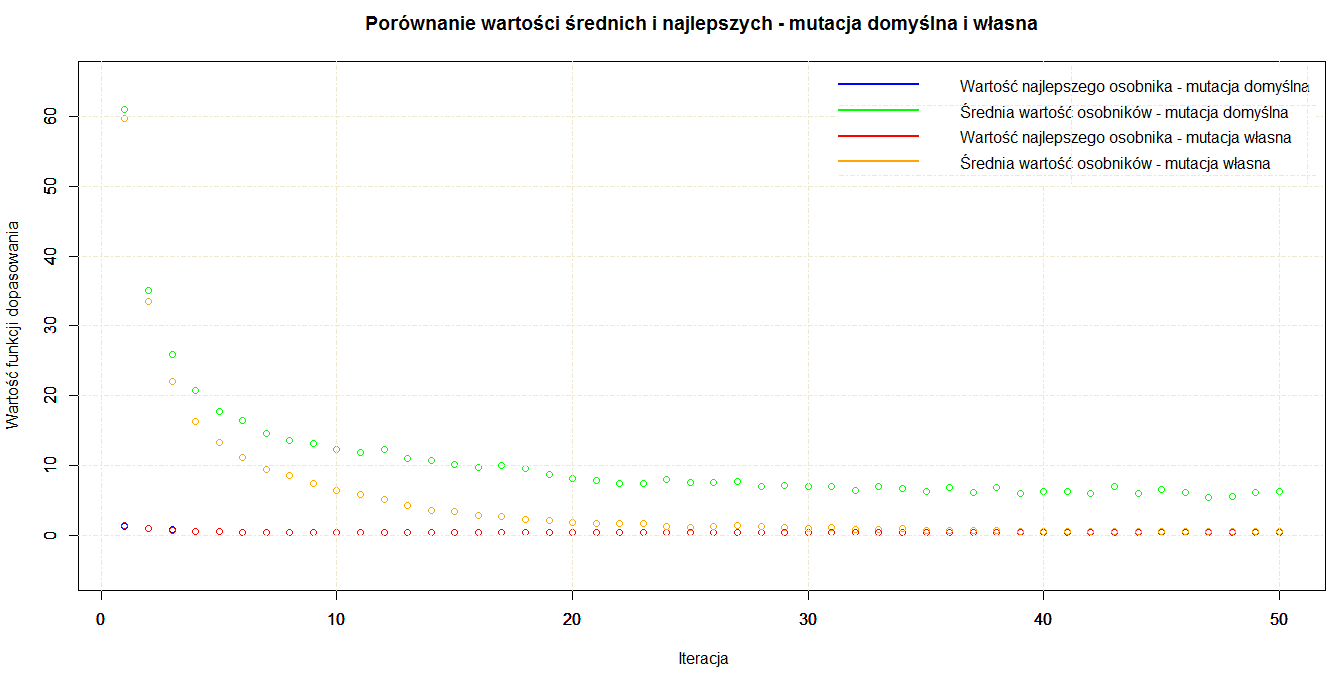
\includegraphics[scale = 0.5]{img/zad1/mut_0_1}
	\caption{Wykres dla prawdopodobieństwa mutacji 0.1}  
	\label{rys:mut_0.1} 
\end{figure}

\begin{figure}[H]
	\centering
	\hspace*{-0.8in}
	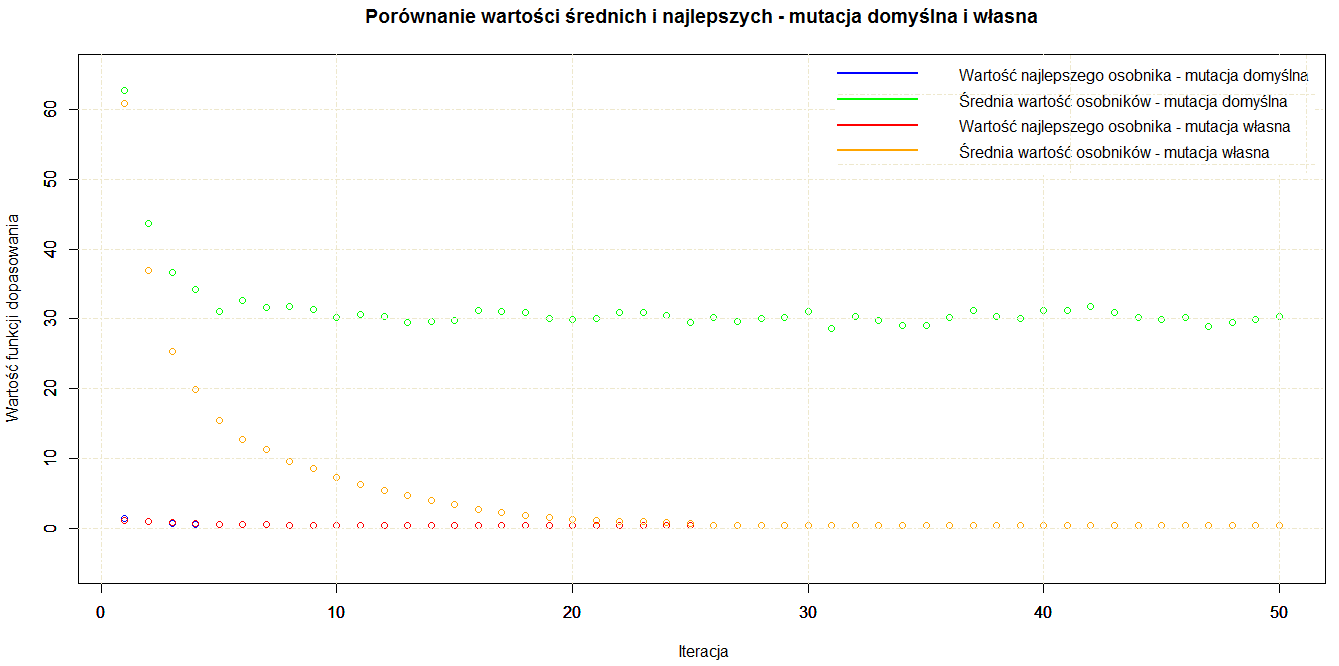
\includegraphics[scale = 0.5]{img/zad1/mut_0_5}
	\caption{Wykres dla prawdopodobieństwa mutacji 0.5}  
	\label{rys:mut_0.5} 
\end{figure}

\begin{figure}[H]
	\centering
	\hspace*{-0.8in}
	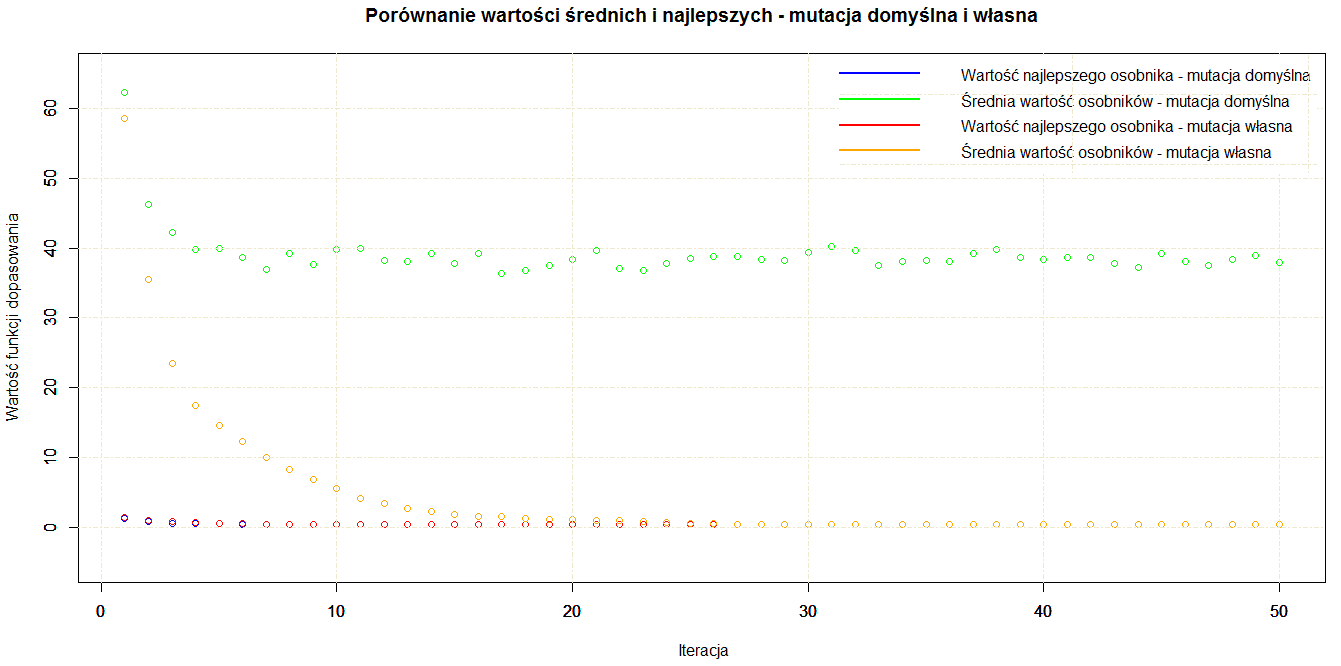
\includegraphics[scale = 0.5]{img/zad1/mut_0_7}
	\caption{Wykres dla prawdopodobieństwa mutacji 0.7}  
	\label{rys:mut_0.7} 
\end{figure}

\begin{figure}[H]
	\centering
	\hspace*{-0.8in}
	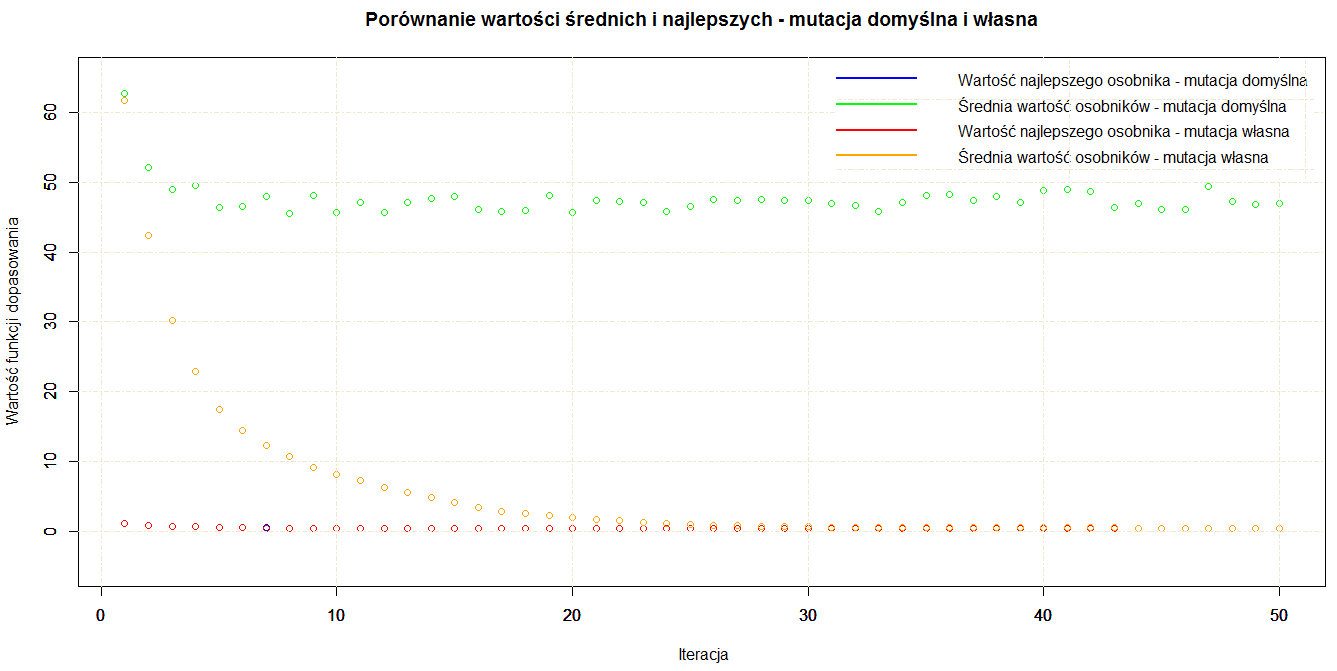
\includegraphics[scale = 0.5]{img/zad1/mut_1}
	\caption{Wykres dla prawdopodobieństwa mutacji 1}  
	\label{rys:mut_1} 
\end{figure}



\subsubsection{Wnioski}

\begin{table}[!h]
	\hspace*{-1.5in}
	\centering
	\caption{Wartości średnie i najlepsze osobnika dla domyślnej i własnej funkcji mutacji}
	\label{mut_porownanie}
	\hspace*{-0.4in}
	\begin{tabular}{|c|c|c|c|c|}
		\hline
		\textbf{Prawdopodobieństwo} & \multicolumn{2}{c}{\textbf{Mutacja domyślna}}  & \multicolumn{2}{|c|}{\textbf{Mutacja własna}} \\ \cline{2-5}
		\textbf{mutacji} & Wartość średnia & Najlepszy wynik & Wartość średnia & Najlepszy wynik \\ \hline
		
		0.1 & 5.753710  & 0.398006 & 0.398736 & 0.398687 \\
		0.5 & 31.029570 & 0.401904 & 0.415733 & 0.398201 \\
		0.7 & 38.184020 & 0.404532 & 0.567679 & 0.398926 \\
		1   & 46.920430 & 0.408154 & 0.452637 & 0.400847  \\ \hline      
	\end{tabular}
\end{table}
\subsection{Selekcja}

\subsubsection{Kod źródłowy}


\subsubsection{Wyniki badań}


\begin{figure}[]
	\centering
	\hspace*{-0.8in}
	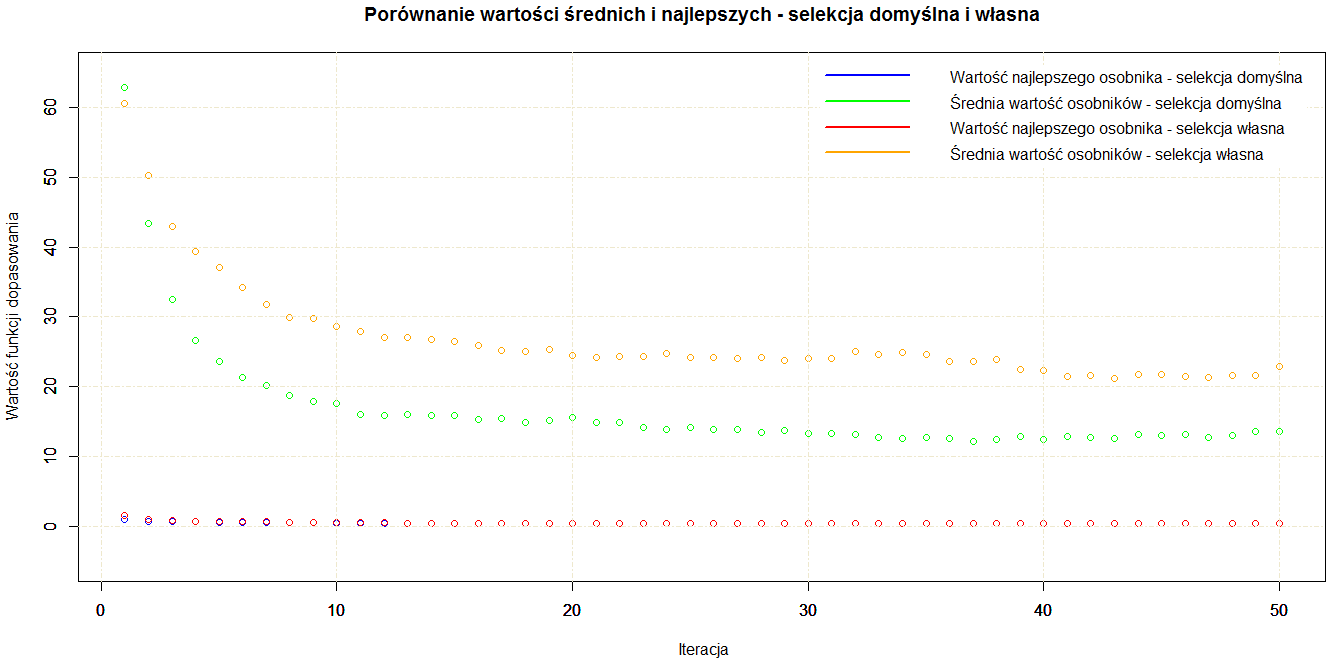
\includegraphics[scale = 0.5]{sel_1}
	\caption{Wykres przy 1 osobniku elitarnym}  
	\label{rys:sel_1} 
\end{figure}

\begin{figure}[H]
	\centering
	\hspace*{-0.8in}
	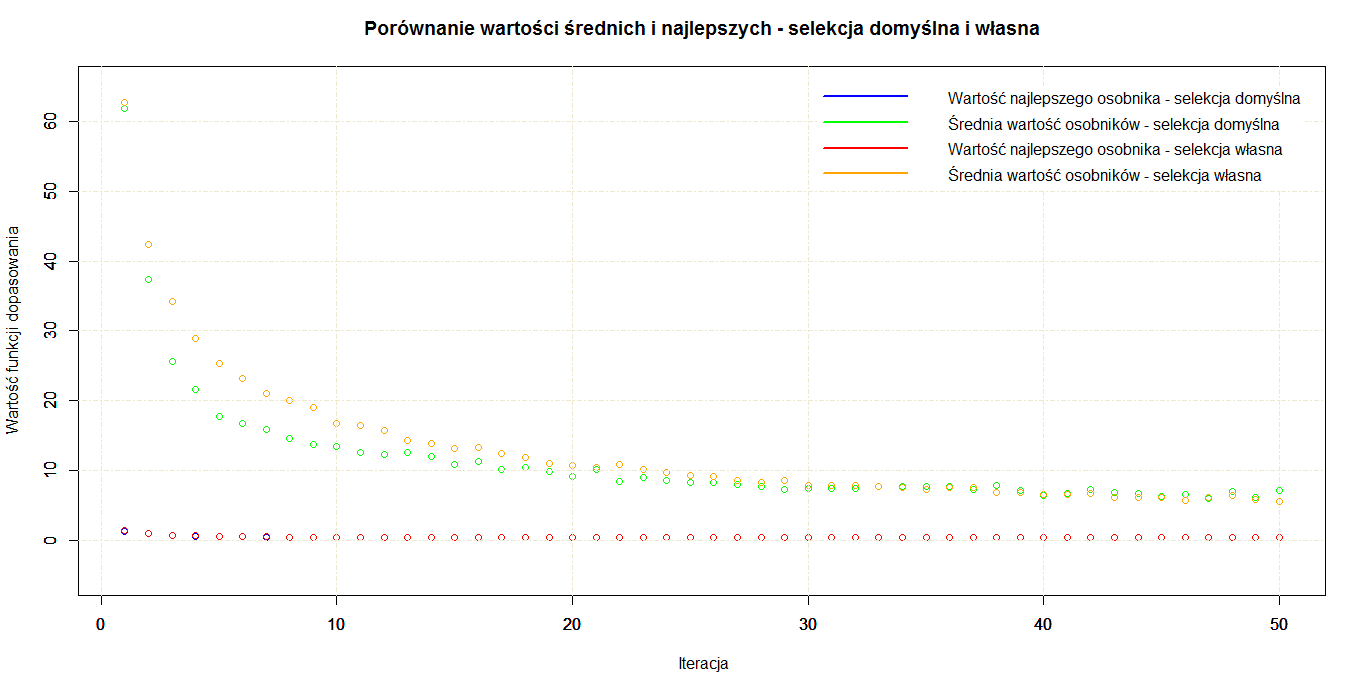
\includegraphics[scale = 0.5]{sel_6}
	\caption{Wykres przy 6 osobnikach elitarnych}  
	\label{rys:sel_6} 
\end{figure}

\begin{figure}[H]
	\centering
	\hspace*{-0.8in}
	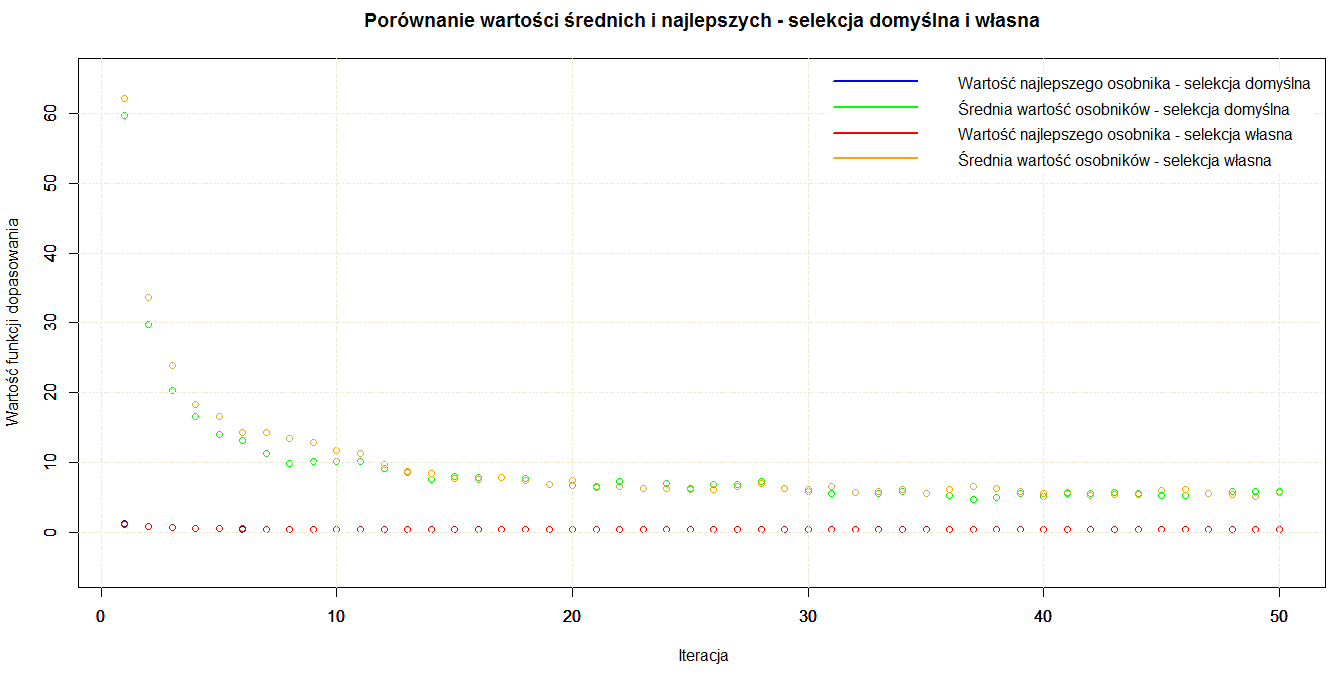
\includegraphics[scale = 0.5]{sel_20}
	\caption{Wykres przy 20 osobnikach elitarnych}  
	\label{rys:sel_20} 
\end{figure}

\begin{figure}[H]
	\centering
	\hspace*{-0.8in}
	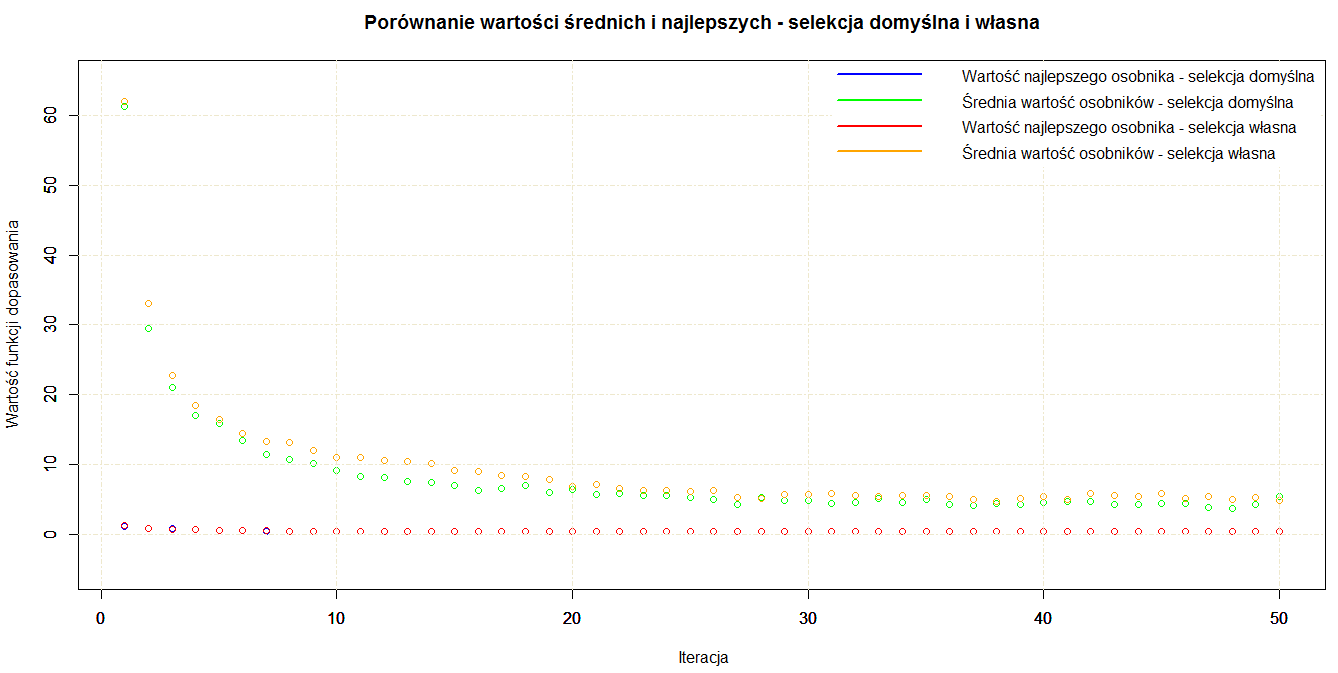
\includegraphics[scale = 0.5]{sel_50}
	\caption{Wykres przy 50 osobnikach elitarnych}  
	\label{rys:sel_50} 
\end{figure}

\subsubsection{Wnioski}

\begin{table}[!h]
	\centering
	\caption{Wartości średnie i najlepsze osobnika dla domyślnej i własnej funkcji selekcji}
	\label{sel_porownanie}
	\begin{tabular}{|c|c|c|c|c|}
		\hline
		\textbf{Selekcja} & \multicolumn{2}{c}{\textbf{Selekcja domyślna}}  & \multicolumn{2}{|c|}{\textbf{Selekcja własna}} \\ \cline{2-5}
		\textbf{elitarna} & Wartość średnia & Najlepszy wynik & Wartość średnia & Najlepszy wynik \\ \hline
		
		1  & 13.660880  & 0.405495 & 22.860800 & 0.414707 \\
		6  & 7.106856 & 0.400895 & 5.544652 & 0.397909 \\
		20 & 5.847374 & 0.397888 & 5.678752 & 0.397977 \\
		50 & 5.42606 & 0.397903 & 4.833812 & 0.397888  \\ \hline      
	\end{tabular}
\end{table}
\newpage
\subsection{Krzyżowanie}

Krzyżowanie jest podstawowym mechanizmem tworzenia potomstwa na podstawie wartości przyjmowanych przez rodziców. W stworzonej implementacji pobierana jest połowa wartości od każdego z nich, a ich suma stanowi nowego potomka

\subsubsection{Kod źródłowy}

\begin{lstlisting}[linewidth=16.0cm]
myCrossover <- function (ga_object, parents)
{
  # Pobranie rodzicow do skrzyzowania
  # i zainicjalizowanie nimi potomstwa
  parents <- ga_object@population[parents,,drop = FALSE]
  parCol <- ncol(parents)
  parRow <- nrow(parents)
  children <- parents

  
  for (i in 1:parCol)
  { 
	for(j in 1:parRow)
	{
	  if (j == parCol) {  
	    nextCol <- 1 
	  }
	  else {
	    nextCol <- j+1
      }
      
      # Resultat krzyzowania - 
      # suma 1/2 wartosci kazdego rodzica z wybranych pol
	  newChild <- parents[i, j]/2 + parents[i, nextCol]/2
	  children[i, j] <- newChild
	}
  }

  out <- list(children = children, fitness = rep(NA,2))
  return(out)
}
\end{lstlisting}

\subsubsection{Wyniki badań}

\begin{figure}[H]
	\centering
	\hspace*{-0.8in}
	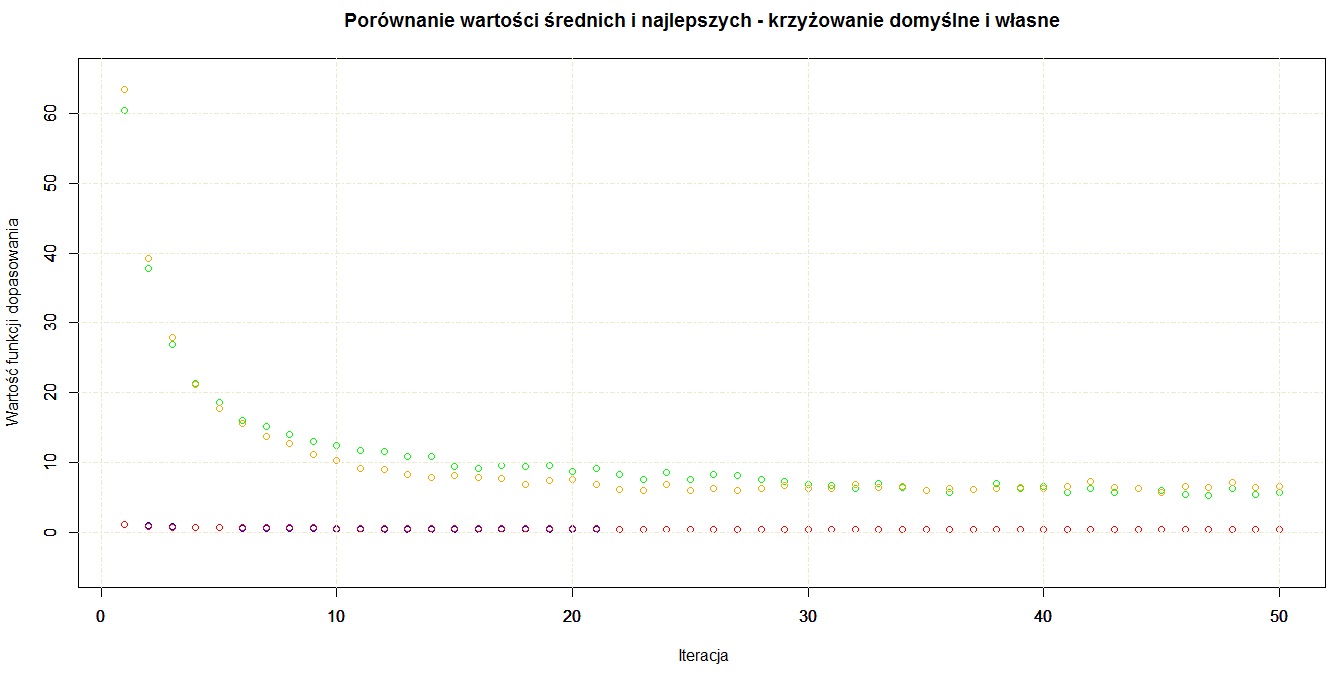
\includegraphics[scale = 0.5]{img/zad1/cross_0_2}
	\caption{Wykres dla prawdopodobieństwa krzyżowania 0.2}  
	\label{rys:cross_0_2} 
\end{figure}


\begin{figure}[H]
	\centering
	\hspace*{-0.8in}
	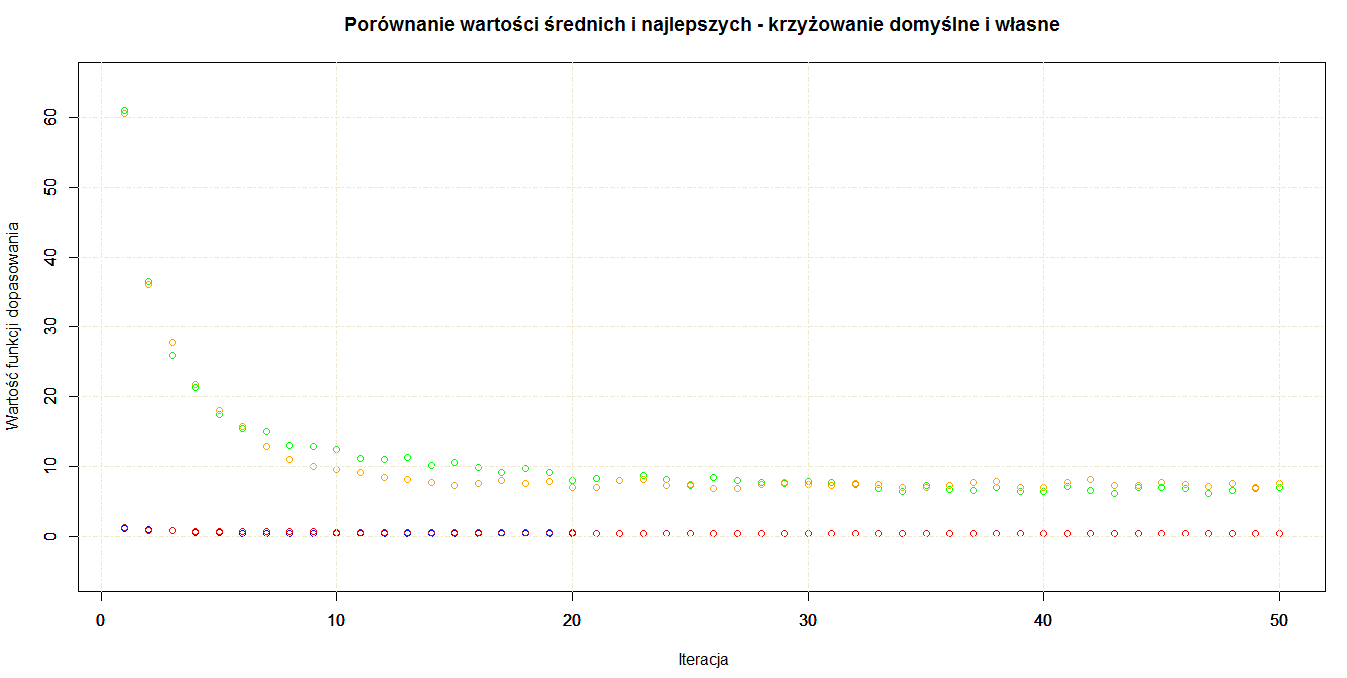
\includegraphics[scale = 0.5]{img/zad1/cross_0_5}
	\caption{Wykres dla prawdopodobieństwa krzyżowania 0.5}  
	\label{rys:cross_0_5} 
\end{figure}


\begin{figure}[H]
	\centering
	\hspace*{-0.8in}
	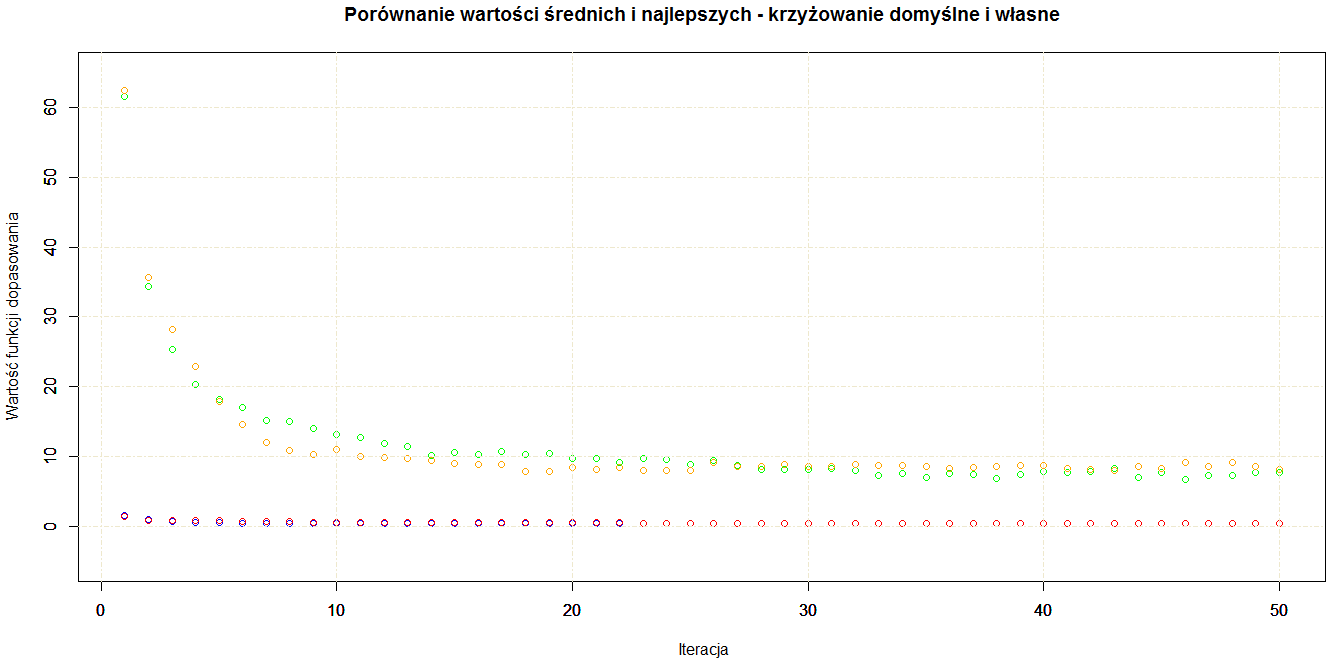
\includegraphics[scale = 0.5]{img/zad1/cross_0_7}
	\caption{Wykres dla prawdopodobieństwa krzyżowania 0.7}  
	\label{rys:cross_0_7} 
\end{figure}


\begin{figure}[H]
	\centering
	\hspace*{-0.8in}
	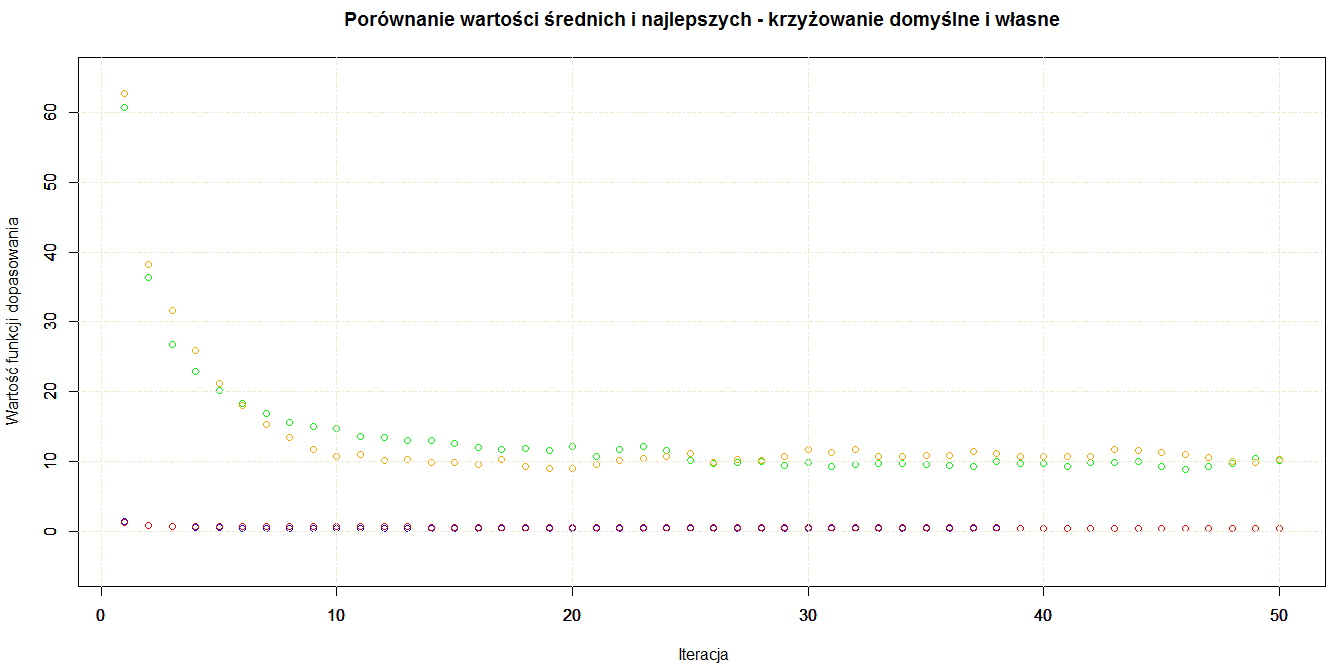
\includegraphics[scale = 0.5]{img/zad1/cross_1}
	\caption{Wykres dla prawdopodobieństwa krzyżowania 1}  
	\label{rys:cross_1} 
\end{figure}

\vline

\subsubsection{Wnioski}

\begin{table}[!h]
	\centering
	\caption{Wartości średnie i najlepsze osobnika dla domyślnej i własnej funkcji krzyżowania}
	\label{cross_porownanie}
	\hspace*{-0.5in}
	\begin{tabular}{|c|c|c|c|c|}
		\hline
		\textbf{Prawdopodobieństwo} & \multicolumn{2}{c}{\textbf{Krzyżowanie domyślne}}  & \multicolumn{2}{|c|}{\textbf{Krzyżowanie własne}} \\ \cline{2-5}
		\textbf{krzyżowania} & Wartość średnia & Najlepszy wynik & Wartość średnia & Najlepszy wynik \\ \hline
		
		0.2 & 5.697605 & 0.399347 & 6.538159 & 0.440933 \\
		0.5 & 6.973119 & \textbf{{\color{green} 0.398064 }} & 7.590295 & 0.457468 \\
		0.7 & 7.753576 & 0.398096 & 8.148286 & 0.464140 \\
		1   & 10.206810 & 0.398485 & 10.375570 & 0.476180  \\ \hline      
	\end{tabular}
\end{table}

Tak jak w przypadku mutacji, krzyżowanie nie wpłynęło na poprawę najlepszego wyniku, wręcz przeciwnie - zwiększanie prawdopodobieństwa krzyżowania coraz bardziej pogarszało otrzymywane wartości. Rezultat najbardziej zbliżony do minimum globalnego został uzyskany dla parametrów domyślnych i wbudowanych funkcji.\\
Średnie populacji dla tych dwóch różnych implementacji przeplatały się, oscylując wokół zbliżonych wartości.

\newpage

\end{document}